\documentclass[10pt,a4paper,fleqn]{article}
\setlength{\oddsidemargin}{-1.4mm}
\setlength{\evensidemargin}{-1.4mm}
\setlength{\textwidth}{162mm}
\setlength{\topmargin}{-12mm}
\setlength{\textheight}{249mm}
\usepackage{amsmath,amssymb,bm,booktabs,array}
\usepackage{xcolor,graphicx,tikz,pgfplots}
\usepackage{url}
% Clickable, breakable URLs using pdfTeX primitives; no hyperref dependency.
\let\plainurl\url
\renewcommand{\url}[1]{\ifdefined\pdfstartlink\leavevmode\pdfstartlink attr{/Border [0 0 0]} user{/Subtype /Link /A << /S /URI /URI (\pdfescapestring{#1}) >>}\plainurl{#1}\pdfendlink\else\plainurl{#1}\fi}
\pgfplotsset{compat=1.18}
\newif\ifmarked
\markedfalse
\definecolor{revisionblue}{RGB}{18,61,130}
\newcommand{\rev}[1]{{\ifmarked\color{revisionblue}\else\color{black}\fi #1}}
\newenvironment{revision}{\begingroup\ifmarked\color{revisionblue}\else\color{black}\fi\nobreak\ignorespaces}{\par\endgroup}
\newcommand{\Eavg}{\overline{\mathcal E}_h}
\newcommand{\Cstep}{\mathcal C}
\newcommand{\Rstep}{\mathcal R}
\newcommand{\mean}[1]{\overline{#1}}
\setlength{\textfloatsep}{14pt plus 3pt minus 2pt}
\setlength{\intextsep}{14pt plus 3pt minus 2pt}
\renewcommand{\topfraction}{0.9}
\renewcommand{\textfraction}{0.08}
\renewcommand{\floatpagefraction}{0.75}
\raggedbottom
\setlength{\emergencystretch}{1em}
\pagestyle{empty}
\makeatletter
\newlabel{eq:ch}{{1}{2}{}{equation.1}{}}
\newlabel{eq:energy}{{2}{2}{}{equation.2}{}}
\newlabel{eq:structure}{{3}{2}{}{equation.3}{}}
\newlabel{eq:step}{{4}{3}{}{equation.4}{}}
\newlabel{eq:fit}{{5}{3}{}{equation.5}{}}
\newlabel{eq:ridge}{{6}{3}{}{equation.6}{}}
\newlabel{eq:candidate}{{7}{3}{}{equation.7}{}}
\newlabel{eq:discreteenergy}{{8}{3}{}{equation.8}{}}
\newlabel{eq:derivatives}{{9}{3}{}{equation.9}{}}
\newlabel{eq:massproj}{{10}{4}{}{equation.10}{}}
\newlabel{eq:accept}{{11}{4}{}{equation.11}{}}
\newlabel{eq:backtrack}{{12}{4}{}{equation.12}{}}
\newlabel{eq:descent}{{13}{4}{}{equation.13}{}}
\newlabel{eq:galerkinenergy}{{14}{5}{}{equation.14}{}}
\newlabel{eq:galerkinlaw}{{15}{5}{}{equation.15}{}}
\newlabel{eq:pidmd}{{16}{5}{}{equation.16}{}}
\newlabel{eq:adaptive}{{17}{5}{}{equation.17}{}}
\newlabel{eq:initial}{{18}{6}{}{equation.18}{}}
\newlabel{eq:errors}{{19}{7}{}{equation.19}{}}
\newlabel{eq:structureerror}{{20}{7}{}{equation.20}{}}
\newlabel{eq:violation}{{21}{7}{}{equation.21}{}}
\newlabel{eq:rectangles}{{22}{7}{}{equation.22}{}}
\newlabel{tab:accuracy}{{1}{8}{}{table.1}{}}
\newlabel{tab:epsilon}{{2}{10}{}{table.2}{}}
\newlabel{tab:mobility}{{3}{10}{}{table.3}{}}
\newlabel{tab:long}{{4}{11}{}{table.4}{}}
\newlabel{tab:timing}{{5}{12}{}{table.5}{}}
\newlabel{eq:cost}{{23}{13}{}{equation.23}{}}
\newlabel{tab:convergence}{{6}{13}{}{table.6}{}}
\newlabel{tab:teacher}{{7}{14}{}{table.7}{}}
\newlabel{tab:finer}{{8}{15}{}{table.8}{}}
\newlabel{tab:crossgrid}{{9}{15}{}{table.9}{}}
\newlabel{tab:deterministic}{{10}{15}{}{table.10}{}}
\newlabel{tab:hyper}{{11}{17}{}{table.11}{}}
\newlabel{tab:shifts}{{12}{17}{}{table.12}{}}
\newlabel{eq:fixedfilterlimit}{{24}{18}{}{equation.24}{}}
\makeatother
\begin{document}
\setcounter{figure}{1}
\begin{figure}[htbp]\centering
\begin{tikzpicture}
\begin{axis}[width=.46\textwidth,height=5.4cm,scale only axis=false,grid=major,grid style={gray!15},tick label style={font=\footnotesize},label style={font=\small},title style={font=\small},legend style={font=\scriptsize,draw=none,fill=white},legend cell align=left,title={(a)},xlabel={$t\times10^3$},ylabel={$\overline{\mathcal E}_h$},scaled y ticks=false,yticklabel style={/pgf/number format/fixed,/pgf/number format/precision=3},legend pos=south west]
\addplot[black,thick,solid,mark=*,mark size=1.8pt,mark repeat=5,mark options={solid}] coordinates {(0,0.246948194) (0.1,0.246894856) (0.2,0.24683977) (0.3,0.246782857) (0.4,0.246724034) (0.5,0.246663215) (0.6,0.246600308) (0.7,0.246535215) (0.8,0.246467835) (0.9,0.246398059) (1,0.246325772) (1.1,0.246250853) (1.2,0.246173176) (1.3,0.246092603) (1.4,0.246008991) (1.5,0.245922189) (1.6,0.245832036) (1.7,0.245738361) (1.8,0.245640983) (1.9,0.24553971) (2,0.24543434) (2.1,0.245324655) (2.2,0.245210428) (2.3,0.245091415) (2.4,0.244967357) (2.5,0.244837981) (2.6,0.244702995) (2.7,0.244562089) (2.8,0.244414936) (2.9,0.244261184) (3,0.244100464) (3.1,0.24393238) (3.2,0.243756514) (3.3,0.24357242) (3.4,0.243379626) (3.5,0.243177628)};\addlegendentry{Reference (100)}
\addplot[orange!85!black,thick,dashed,mark=square*,mark size=1.8pt,mark repeat=5,mark options={solid}] coordinates {(0,0.246948194) (0.1,0.246897258) (0.2,0.246844787) (0.3,0.246790721) (0.4,0.246734995) (0.5,0.246677544) (0.6,0.246618296) (0.7,0.246557179) (0.8,0.246494117) (0.9,0.246429027) (1,0.246361827) (1.1,0.246292428) (1.2,0.246220737) (1.3,0.246146656) (1.4,0.246070085) (1.5,0.245990915) (1.6,0.245909036) (1.7,0.245824328) (1.8,0.245736668) (1.9,0.245645928) (2,0.245551969) (2.1,0.24545465) (2.2,0.24535382) (2.3,0.245249322) (2.4,0.24514099) (2.5,0.24502865) (2.6,0.244912119) (2.7,0.244791205) (2.8,0.244665708) (2.9,0.244535415) (3,0.244400103) (3.1,0.24425954) (3.2,0.24411348) (3.3,0.243961666) (3.4,0.243803827) (3.5,0.243639679)};\addlegendentry{Uncorrected (1)}
\addplot[blue!65!black,thick,densely dotted,mark=diamond*,mark size=1.8pt,mark repeat=5,mark options={solid}] coordinates {(0,0.246948194) (0.1,0.246894864) (0.2,0.246839787) (0.3,0.246782883) (0.4,0.246724073) (0.5,0.246663267) (0.6,0.246600376) (0.7,0.246535302) (0.8,0.246467942) (0.9,0.246398191) (1,0.246325932) (1.1,0.246251047) (1.2,0.246173407) (1.3,0.246092879) (1.4,0.246009318) (1.5,0.245922576) (1.6,0.245832491) (1.7,0.245738894) (1.8,0.245641607) (1.9,0.24554044) (2,0.24543519) (2.1,0.245325645) (2.2,0.245211578) (2.3,0.245092748) (2.4,0.244968902) (2.5,0.244839767) (2.6,0.244705058) (2.7,0.24456447) (2.8,0.244417679) (2.9,0.244264342) (3,0.244104095) (3.1,0.24393655) (3.2,0.243761298) (3.3,0.243577903) (3.4,0.243385902) (3.5,0.243184806)};\addlegendentry{Residual (6)}
\end{axis}
\end{tikzpicture}
\hfill
\begin{tikzpicture}
\begin{axis}[width=.46\textwidth,height=5.4cm,scale only axis=false,grid=major,grid style={gray!15},tick label style={font=\footnotesize},label style={font=\small},title style={font=\small},legend style={font=\scriptsize,draw=none,fill=white},legend cell align=left,title={(b)},xlabel={$t\times10^3$},ylabel={$e_{L^2}$},ymode=log,legend pos=south east]
\addplot[orange!85!black,thick,dashed,mark=square*,mark size=1.8pt,mark repeat=5,mark options={solid}] coordinates {(0.1,0.000913561173) (0.2,0.00186983559) (0.3,0.00287051448) (0.4,0.00391734088) (0.5,0.00501210954) (0.6,0.00615666664) (0.7,0.00735290916) (0.8,0.00860278409) (0.9,0.00990828716) (1,0.0112714614) (1.1,0.0126943951) (1.2,0.0141792195) (1.3,0.015728106) (1.4,0.017343263) (1.5,0.0190269314) (1.6,0.020781381) (1.7,0.0226089046) (1.8,0.0245118126) (1.9,0.0264924264) (2,0.0285530712) (2.1,0.0306960675) (2.2,0.0329237225) (2.3,0.0352383199) (2.4,0.0376421094) (2.5,0.0401372944) (2.6,0.0427260196) (2.7,0.045410357) (2.8,0.0481922911) (2.9,0.0510737028) (3,0.0540563528) (3.1,0.0571418634) (3.2,0.0603316995) (3.3,0.063627149) (3.4,0.0670293022) (3.5,0.0705390298)};\addlegendentry{Uncorrected (1)}
\addplot[teal!80!black,thick,dashdotted,mark=triangle*,mark size=1.8pt,mark repeat=5,mark options={solid}] coordinates {(0.1,0.000158765299) (0.2,0.000325813885) (0.3,0.000501533767) (0.4,0.000686328926) (0.5,0.000880619643) (0.6,0.00108484279) (0.7,0.00129945205) (0.8,0.00152491812) (0.9,0.00176172884) (1,0.00201038916) (1.1,0.00227142119) (1.2,0.00254536396) (1.3,0.00283277321) (1.4,0.00313422103) (1.5,0.00345029526) (1.6,0.0037815989) (1.7,0.00412874921) (1.8,0.0044923767) (1.9,0.00487312393) (2,0.00527164401) (2.1,0.00568859896) (2.2,0.00612465777) (2.3,0.00658049418) (2.4,0.00705678419) (2.5,0.00755420325) (2.6,0.00807342315) (2.7,0.00861510856) (2.8,0.00917991319) (2.9,0.00976847564) (3,0.0103814148) (3.1,0.011019325) (3.2,0.0116827706) (3.3,0.0123722803) (3.4,0.013088341) (3.5,0.0138313914)};\addlegendentry{Uncorrected (6)}
\addplot[purple,thick,dashdotdotted,mark=pentagon*,mark size=1.8pt,mark repeat=5,mark options={solid}] coordinates {(0.1,7.5078925e-05) (0.2,0.000154124383) (0.3,0.000237325824) (0.4,0.00032488075) (0.5,0.000416994894) (0.6,0.000513882393) (0.7,0.000615765927) (0.8,0.000722876832) (0.9,0.000835455186) (1,0.000953749857) (1.1,0.0010780185) (1.2,0.00120852754) (1.3,0.00134555202) (1.4,0.0014893755) (1.5,0.0016402898) (1.6,0.00179859472) (1.7,0.0019645976) (1.8,0.00213861292) (1.9,0.00232096167) (2,0.00251197067) (2.1,0.00271197177) (2.2,0.00292130092) (2.3,0.00314029709) (2.4,0.00336930108) (2.5,0.00360865408) (2.6,0.00385869622) (2.7,0.0041197648) (2.8,0.00439219239) (2.9,0.00467630479) (3,0.00497241874) (3.1,0.00528083942) (3.2,0.0056018578) (3.3,0.00593574775) (3.4,0.00628276293) (3.5,0.00664313355)};\addlegendentry{Uncorrected (12)}
\addplot[blue!65!black,thick,densely dotted,mark=diamond*,mark size=1.8pt,mark repeat=5,mark options={solid}] coordinates {(0.1,4.68504749e-05) (0.2,9.82875283e-05) (0.3,0.000154629588) (0.4,0.000216211513) (0.5,0.000283385014) (0.6,0.000356519053) (0.7,0.000436000196) (0.8,0.000522232925) (0.9,0.000615639898) (1,0.000716662146) (1.1,0.000825759208) (1.2,0.000943409186) (1.3,0.00107010871) (1.4,0.00120637282) (1.5,0.00135273472) (1.6,0.00150974543) (1.7,0.00167797329) (1.8,0.00185800338) (1.9,0.00205043668) (2,0.00225588914) (2.1,0.00247499057) (2.2,0.00270838327) (2.3,0.00295672054) (2.4,0.00322066487) (2.5,0.00350088596) (2.6,0.00379805847) (2.7,0.0041128595) (2.8,0.00444596579) (2.9,0.00479805065) (3,0.00516978061) (3.1,0.00556181167) (3.2,0.00597478542) (3.3,0.00640932465) (3.4,0.00686602882) (3.5,0.00734546908)};\addlegendentry{Residual (6)}
\end{axis}
\end{tikzpicture}

\rev{\caption{\rev{Representative main-test trajectory (index zero) on the legacy periodic $64^2$ grid, with $\epsilon=0.020$, $M=1$ and macro step $10^{-4}$. (a) Area-averaged monitored energy: the 100-substep reference is black with a solid line and circles; the one-substep method is orange with a dashed line and squares; the six-substep residual surrogate is blue with a dotted line and diamonds. (b) Relative field error against the 100-substep reference: one, six and twelve uncorrected substeps use orange dashed squares, teal dash-dot triangles and purple dash-dot-dot pentagons; the residual surrogate uses blue dotted diamonds. The horizontal axis displays $10^3t$. Markers are spaced for legibility; all plotted samples are retained. These are individual trajectories, not ensemble means.}}\label{fig:trajectories}}
\end{figure}
\clearpage
\end{document}
